\section{Auswertung}
\label{sec:Auswertung}

Zunächst wird eine Justage für eine möglichst große Amplitude des FID und eine Minimierung des Imaginärteils durchgeführt. 
Diese führt zu folgenden Werten

\begin{align}
  \omega_\text{L} &= \SI{21.72573}{\mega\hertz},\\
  \phi &= \SI{32}{\degree}
\end{align}

für die Lamorfrequenz $\omega_\text{L}$ und die Phase $\phi$. Die Pulslängen des $\SI{90}{\degree}$ und des $\SI{180}{\degree}$
ergeben sich zu 

\begin{align}
  \symup{\Delta} t_{90} &= \SI{2.68}{\micro\second},\\
  \symup{\Delta} t_{180} &= \SI{5.02}{\micro\second}.
\end{align}

Die Temperaturmessungen zu Beginn der Messungen und als Abschluss dieser, ergeben als Temperaturen innerhalb des Magneten: 

\begin{align}
  T_\text{Beginn} &= \SI{19.5}{\celsius},\\
  T_\text{Ende} &= \SI{22.2}{\celsius}.
\end{align}

\subsection{Bestimmung der Spin-Gitter Relaxationszeit}

In diesem Abschnitt soll die Spin-Gitter Relaxationszeit $T_1$ bestimmt werden. Hierzu wurde die Spannungsamplitude der 
induzierten Spannung für verschiedene Pulsabstände $\tau$ gemessen. Die Messwerte sind in Tabelle \ref{tab:mess1} zu finden.

\begin{table}
  \centering
  \caption{Messwerte zur Bestimmung der Relaxationszeit $T_1$. Es wurde die Spannungsamplitude $U$ für verschiedene Pulsabstände $\tau$ gemessen.}
  \label{tab:mess1}
  \sisetup{table-format=2.1}
  \begin{tabular}{c c c c}
  \toprule
  $\tau \,/\, \si{\milli\second}$ & $U \,/\, \si{\volt}$ & $\tau \,/\, \si{\milli\second}$
  & $U \,/\, \si{\volt}$\\
  \midrule 
        1,0 & -1,8813 &  155,6 & -1,3188\\
        1,4 & -1,7125 &  217,8 & -1,1813\\
        2,0 & -1,7938 &  309,4 & -1,1063\\
        2,7 & -1,7438 &  426,9 & -1,0875\\
        3,8 & -1,7875 &  597,6 & -0,9313\\
        5,4 & -1,6563 & 1172,3 & -0,4375\\
        7,5 & -1,7125 & 1639,9 & -0,0650\\
       10,5 & -1,6000 & 2295,9 &  0,2588\\
       14,8 & -1,6875 & 3214,3 &  0,7250\\
       28,9 & -1,6250 & 4500,0 &  0,3375\\
       40,5 & -1,6125 & 6300,0 &  0,2950\\
       56,7 & -1,6000 & 7550,0 &  0,3180\\
      111,1 & -1,3375 & 8820,0 &  0,3260\\
  \bottomrule
  \end{tabular}
\end{table}

Diese Messwerte wurden graphisch dargestellt in Abbildung \ref{fig:plot1}. 

\begin{figure}
  \centering
  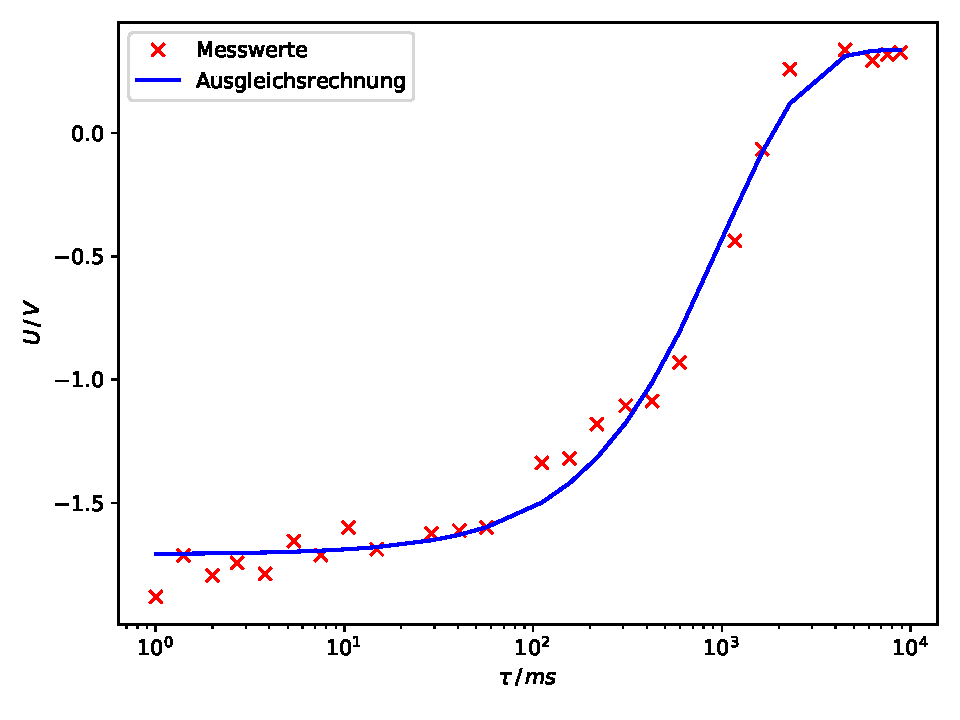
\includegraphics[scale=0.7]{content/plot1.pdf}
  \caption{Halblogarithmische Darstellung der Messwerte mit Ausgleichsrechnung.}
  \label{fig:plot1}
\end{figure}

Mit der Gleichung \eqref{eqn:SGR} wird eine Ausgleichsrechnung
anhand von 

\begin{equation*}
  U\left(\tau\right) = U_0 \left(1-2\exp{\left(-\frac{\tau}{T_1}\right)}\right) + U_1
\end{equation*}

durchgeführt. Dabei dient $U_1$ zum Ausgleich der Nulllinie. 
Die Parameter der Ausgleichsrechnung ergeben sich mittels \textit{python} zu:

\begin{align}
  U_0 &= \SI{1.023(25)}{\volt},\\
  T_1 &= \SI{1.03(8)e3}{\milli\second},\\
  U_1 &= \SI{-0.685(27)}{\volt}.
\end{align}

\subsection{Bestimmung der Spin-Spin Relaxationszeit}

Die Bestimmung der Relaxationszeit $T_2$ erfolgt mithilfe der Meiboom-Gill-Methode. Anschließend wird die Carr-Purcell-Methode 
betrachtet, die allerdings kein Ergebnis für $T_2$ liefern kann.

\subsubsection{Meiboom-Gill-Methode}

Das von der Meiboom-Gill Methode gelieferte Signal ist in Abbildung \ref{fig:mgm} zu sehen. 

\begin{figure}
  \centering
  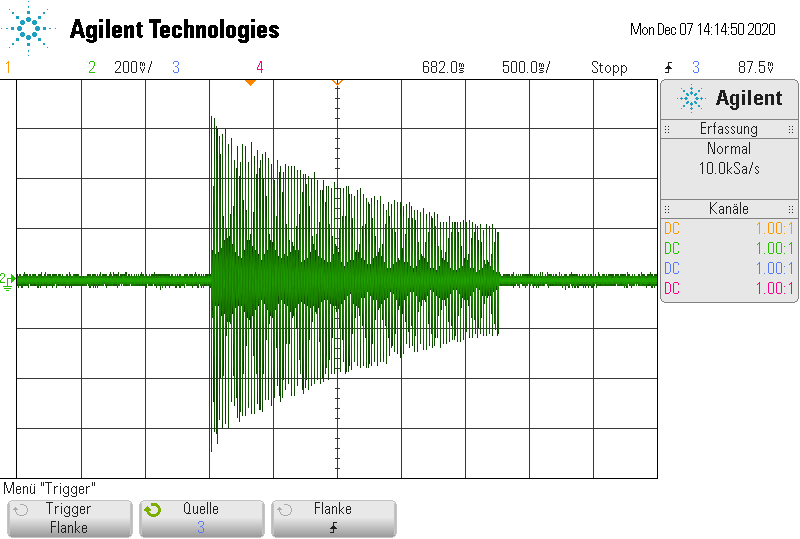
\includegraphics[scale=0.4]{content/mgm.png}
  \caption{Dises Signal wurde mithilfe der Meiboom-Gill-Methode aufgenommen.}
  \label{fig:mgm}
\end{figure}

Mithilfe der Funktion \textit{scipy.signal.find\_peaks}\cite{scipy} 
werden die Peaks mit positiver Spannungsamplitude $U$ aus dem Signal herausgefiltert. Die Bestimmung der Peaks erfolgt 
dabei über die CSV-Datei des Signals. Hierbei ist zu erwähnen, dass weniger als die erwarteten $100$ Peaks extrahiert werden 
konnten.
Die so erhaltenen Messwerte sind in Tabelle \ref{tab:mess2} aufgeführt und in Abbildung \ref{fig:plot2} 
graphisch dargestellt. 

\begin{table}
  \centering
  \caption{Herausgefilterte Peaks des Signals zur Bestimmung von $T_2$.}
  \label{tab:mess2}
  \sisetup{table-format=2.1}
  \begin{tabular}{c c}
  \toprule
  $t \,/\, \si{second}$ & $U \,/\, \si{\volt}$\\
  \midrule 
      -0,19 & 0,60251\\
      -0,01 & 0,40101\\
       0,14 & 0,44171\\
       0,32 & 0,42563\\
       0,62 & 0,33719\\
       0,86 & 0,36131\\
       1,04 & 0,29699\\
       1,29 & 0,24874\\
       1,60 & 0,20854\\
       1,80 & 0,14472\\
  \bottomrule
  \end{tabular}
\end{table}

\begin{figure}
  \centering
  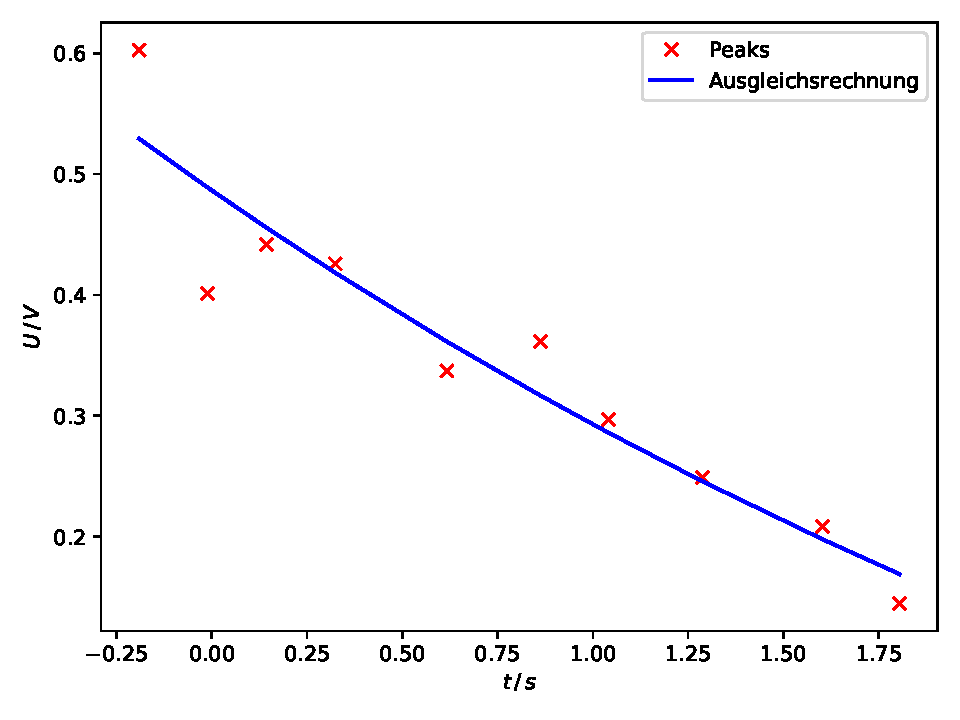
\includegraphics[scale=0.7]{content/plot2.pdf}
  \caption{Anhand der extrahierten Peaks wurde eine Ausgleichsrechnung zur Bestimmung von $T_2$ durchgeführt.}
  \label{fig:plot2}
\end{figure}

Mit der Gleichung \eqref{eqn:MGM} wird eine Ausgleichsrechnung anhand von 

\begin{equation*}
  U\left(t\right) = U_0 \exp{\left(-\frac{t}{T_2}\right)} + U_2
\end{equation*}

durchgeführt, wobei $t = 2\tau$ gilt und $U_2$ die Verschiebung der Nulllinie ist. 

Die Parameter der Ausgleichsrechnung ergeben sich mittels \textit{python} zu:

\begin{align}
  U_0 &= \SI{0.9(14)}{\volt},\\
  T_2 &= \SI{4(8)}{\second},\\
  U_2 &= \SI{-0.4(14)}{\volt}.
\end{align}

\subsubsection{Carr-Purcell-Methode}

Um genaue Ergebnisse zu erhalten, ist eine exakte Einstellung der Pulslänge für den $\SI{180}{\degree}$-Puls notwendig. Dies ist 
in der Praxis nicht umsetzbar und würde zu großen Fehlern führen. Es ergibt sich aus dieser Methode demnach lediglich ein Signal,
das in Abbildung \ref{fig:cpm} zu sehen ist. $T_2$ kann daraus nicht bestimmt werden.  

\begin{figure}
  \centering
  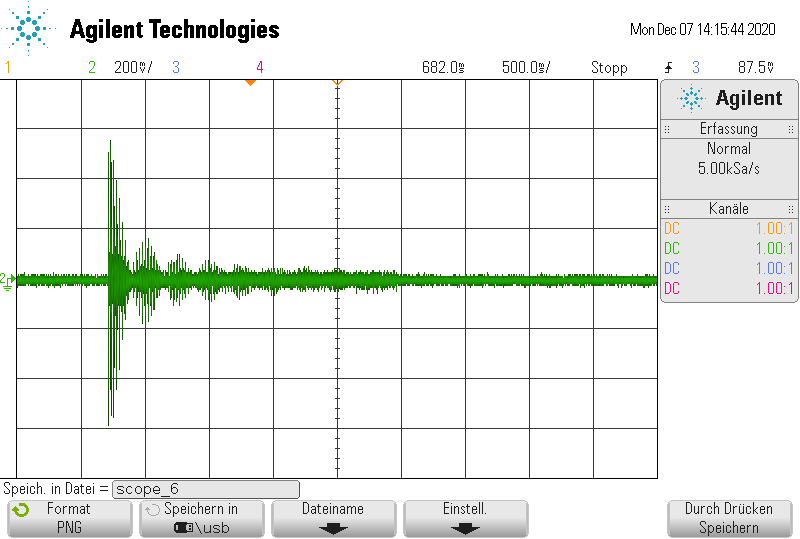
\includegraphics[scale=0.4]{content/scope_6.png}
  \caption{Mit der Carr-Purcell-Methode aufgenommenes Signal.}
  \label{fig:cpm}
\end{figure}

\subsection{Bestimmung der Magnetfeldgradientenstärke}

Zur Bestimmung der Gradientenstärke $G$ wird das gut sichbare Echo in Abbildung \ref{fig:mfg} fouriertransformiert.

\begin{figure}
  \centering
  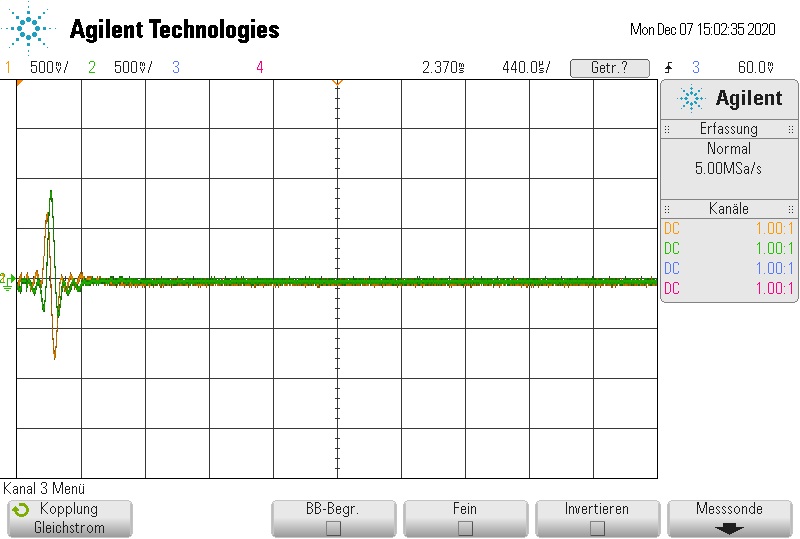
\includegraphics[scale=0.4]{content/scope_8.png}
  \caption{Verwendetes Echo zur Bestimmung der Magnetfeldgradientenstärke.}
  \label{fig:mfg}
\end{figure}

Die Fouriertransformation erfolgt mittels \textit{numpy}\cite{numpy} und ergibt ein Spektrum, welches in Abbildung \ref{fig:trafoecho} zu sehen ist. 

\begin{figure}
  \centering
  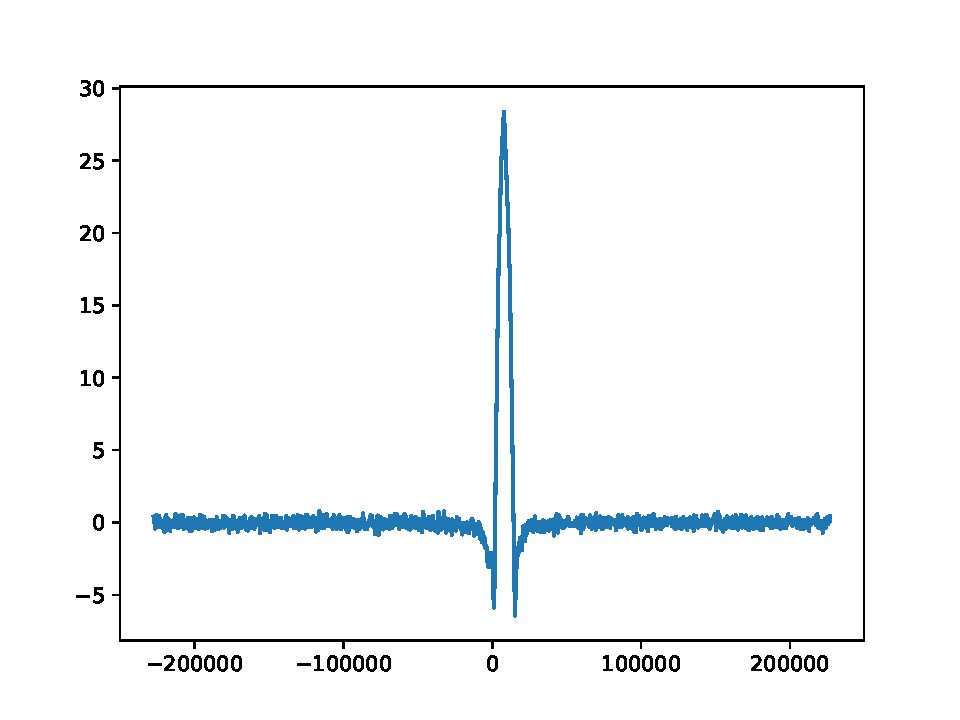
\includegraphics[scale=0.7]{content/echo_gradient.pdf}
  \caption{Vollständige Transformation des Echos.}
  \label{fig:trafoecho}
\end{figure}

Mit dem Durchmesser des Proberöhrchens $d = \SI{4.2}{\milli\metre}$, dem gyromagnetischem Verhältnis für Protonen 
$\gamma = \SI{2.67e8}{\per\second\tesla}$ und dem Durchmesser des Halbkreises im Spektrum des Echos $d_\text{f} \approx \SI{14040}{\hertz}$
ergibt sich $G$ zu 

\begin{equation*}
  G = \frac{2\pi d_\text{f}}{\gamma d} = \SI{0.079}{\tesla\per\metre}.
\end{equation*}

\subsection{Bestimmung der Diffusionskonstante}

Zur Bestimmung der Diffusionskonstante $D$ werden die gemessenen Spannungsamplituden $U$ für verschiedene Pulsabstände $\tau$ aus 
Tabelle \ref{tab:mess3} in Abbildung \ref{fig:plot4} graphisch dargestellt.  

\begin{table}
  \centering
  \caption{Gemessene Spannungsamplituden $U\left(\tau\right)$ zur Bestimmung der Diffusionskonstante $D$.}
  \label{tab:mess3}
  \sisetup{table-format=2.1}
  \begin{tabular}{c c c c}
  \toprule
  $\tau \,/\, \si{\milli\second}$ & $U \,/\, \si{\volt}$ & $\tau \,/\, \si{\milli\second}$
  & $U \,/\, \si{\volt}$\\
  \midrule 
       0,1 & 1,1625 & 11,0 & 0,5813\\
       1,0 & 1,1750 & 12,0 & 0,4500\\
       2,0 & 1,1625 & 13,0 & 0,3425\\
       3,0 & 1,1625 & 14,0 & 0,2375\\
       4,0 & 1,1375 & 15,0 & 0,1775\\
       5,0 & 1,1125 & 16,0 & 0,1250\\
       6,0 & 1,0625 & 17,0 & 0,1025\\
       7,0 & 1,0005 & 18,0 & 0,0713\\
       8,0 & 0,9188 & 19,0 & 0,0575\\
       9,0 & 0,7875 & 20,0 & 0,0500\\
      10,0 & 0,6750 &  & \\
  \bottomrule
  \end{tabular}
\end{table}

Mit der Gleichung \eqref{eqn:DK} wird eine Ausgleichsrechnung anhand von 

\begin{equation*}
  U\left(2\tau\right) = U_0 \exp{\left(-\frac{2\tau}{T_2}\right)} \exp{\left(-\frac{\tau^3}{T_D}\right)} + U_3
\end{equation*}

durchgeführt. 

\begin{figure}
  \centering
  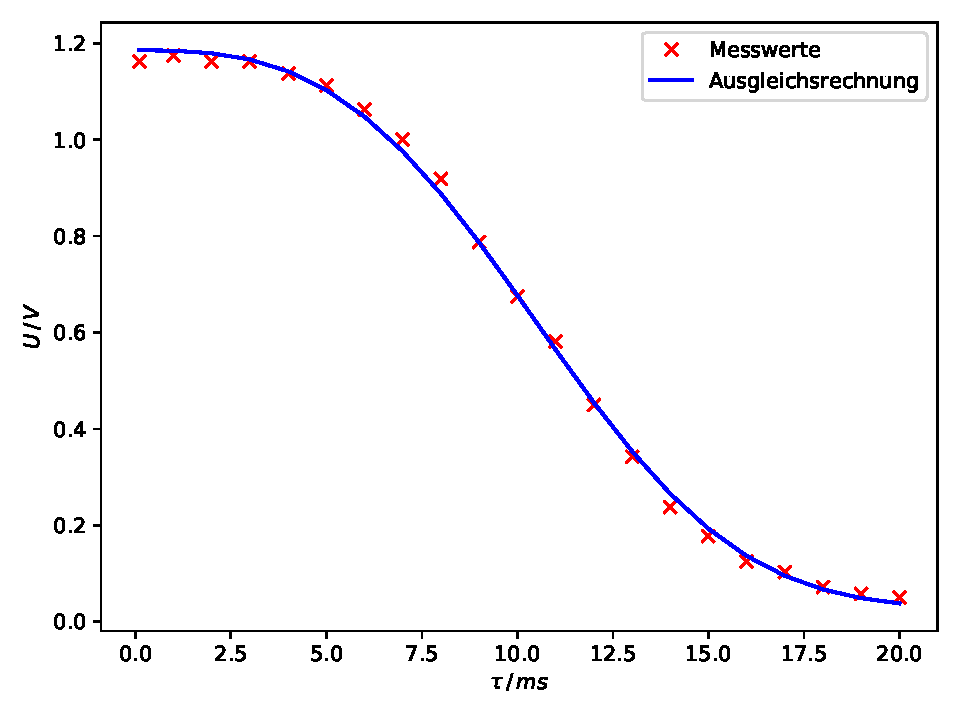
\includegraphics[scale=0.7]{content/plot4.pdf}
  \caption{Spannungsamplitude aufgetragen gegen verschiedene Pulsabstände $\tau$.}
  \label{fig:plot4}
\end{figure}

Die Parameter der Ausgleichsrechnung ergeben sich mittels \textit{python} zu:

\begin{align}
  U_0 &= \SI{1.16(1)}{\volt},\\
  T_D &= \SI{1.75(5)e3}{\milli\second^3},\\
  U_3 &= \SI{0.026(10)}{\volt}.
\end{align}

Mit Gleichung \eqref{eqn:DK} folgt für die Diffusionskonstante

\begin{equation*}
  D = \frac{3}{2\cdot T_D \gamma^2 G^2} = \SI{1.93(5)e-9}{\metre^2\per\second}
\end{equation*}

Um die $\tau^3$-Abhängigkeit zu überprüfen kann noch eine lineare Regression mit 

\begin{equation}
  \ln{\left(U\left(\tau\right)\right)}-\frac{2\tau}{T_2} = a\tau^3+b
\end{equation}

durchgeführt werden. Dies ist in Abbildung \ref{fig:plot5} zu sehen. 

\begin{figure}
  \centering
  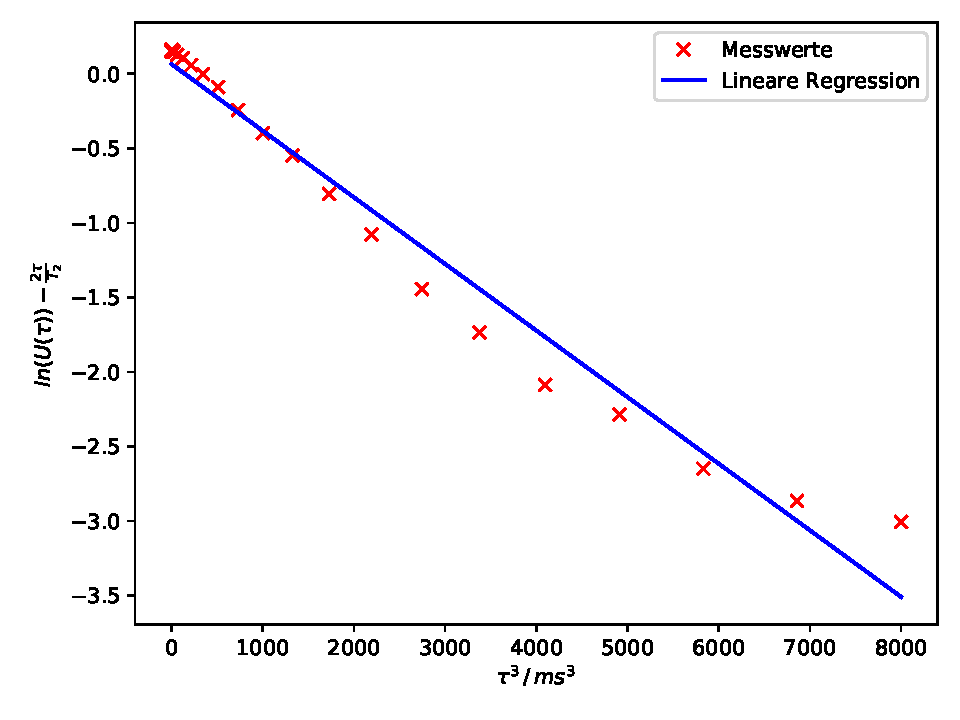
\includegraphics[scale=0.7]{content/plot5.pdf}
  \caption{Lineare Regression zur Kontrolle der $\tau^3$-Abhängigkeit.}
  \label{fig:plot5}
\end{figure}

Die Regressionsparameter ergeben sich zu 

\begin{align*}
  a &= \SI{-0.000447(17)}{\per\milli\second^3},\\
  b &= \num{0.065(54)},
\end{align*}

womit die $\tau^3$-Abhängigkeit in etwa bestätigt werden kann.

\subsection{Bestimmung des Molekülradius}

Der Molekülradius kann mithilfe der Stokes-Formel bestimmt werden:

\begin{equation*}
  D = \frac{k_\text{B}T}{6\pi\eta r} \rightleftarrows r = \frac{k_\text{B}T}{6 \pi\eta D}.
\end{equation*}

Mit $T = \SI{295.35}{\kelvin}$ und einer Viskosität $\eta = \SI{890.2}{\micro\pascal\second}$\cite{vis} ergibt sich ein Molekülradius
von

\begin{equation}
  r = \SI{1.258(33)e-10}{\metre}.
\end{equation}

Zur Berechnung eines Vergleichwertes wird angenommen, dass die Molküle in einer hexagonal dichtesten Kugelpackung angeordnet 
sind. Die Raumfüllung beträgt dort $\SI{74}{\percent}$. Mit einer Molekülmasse von $m = \frac{M_\text{mol}}{N_\text{A}} = \SI{2.99e-26}{\kilo\gram}$
und einer Dichte von $\rho=\SI{995}{\kilo\gram\per\metre^3}$\cite{rho} ergibt sich

\begin{equation}
  r_\text{hcp} = \left(\frac{m\cdot 0.74}{\frac{4}{3}\pi\rho}\right)^{\frac{1}{3}} = \SI{1.74e-10}{\metre}.
\end{equation}

